Reinforcement learning (RL) is a topic in machine learning where \textit{agents} are trained to learn decisions through environment interaction, as visualised in \autoref{fig:RL_model}. A \textit{reward function} indicates the solution's optimality, leading the agent to converge to an optimal policy, where the actions that maximise reward are known for each state. For the problem of robust and optimal rocket landing control, RL presents a promising solution to handling the dynamic and uncertain atmosphere environment and managing high-dimensional control tasks. Unlike traditional model-based methods, deep reinforcement learning uses a neural network as a function approximator to create a model-free control, if done right, with the ability to adapt to uncertainties and unseen scenarios.

\begin{figure}[H]
    \centering
    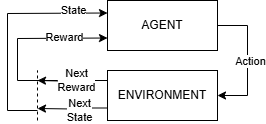
\includegraphics[width=0.65\linewidth]{figures/LiteratureStudy/RL_diagram_basic.png}
    \caption{Reinforcement Learning Model}
    \label{fig:RL_model}
\end{figure}

The aim of the section is to explain the theory behind methods of model-free, off-policy and online learning RL methods, and to survey techniques which can be used to help stabilise and speed up learning, before evaluating the best choice to move forward with. First, the foundations to give the reader a foundation in DRL, Q-learning is explained in \autoref{sec:Q_learning}. Then types of replay buffers are documented in \autoref{sec:buffers} to allow for off-policy learning. As exploration is key to unlocking new control strategies for the agent, a literature review of exploration strategies relevant for this problem is done in \autoref{sec:exploration}. Following this, the algorithms used for learning a problem of our specification are provided in \autoref{sec:off_policy}. Types of mathematical normalisation functions are analysed in \autoref{sec:normalisation_functions} to aide the stability and efficiency of training. Finally, the initial algorithm options are selected in \autoref{sec:RL_algo_selection}.

\subsection{Q-learning}
\label{sec:Q_learning}
A value-based algorithm with an agent learning values of action-state pairs to choose the resulting actions to maximise rewards, \cite{watkins1992q}. This is an off-policy algorithm, so it learns the optimal policy independent of the agent's actions, allowing for model-free RL, as the agent learns the optimal action-value function \(Q^*(s, a)\) through interacting with the environment, providing the maximum expected rewards \(R(s_t, a_t)\) from acting \(a_t\) in the state \(s_t\). The function is updated through \autoref{eq:Qlearning}, where the parameters of the Q-network are updated periodically to equal those of the target network. Here, the discount $\gamma$ determines the importance of future rewards, and $\tau$ affects how quickly new information is learnt.


\begin{equation}
    Q(s_t, a_t; \theta) \leftarrow Q(s_t, a_t; \theta) + \tau [ R(s_t, a_t) + \gamma \max_{a_{t+1}} Q(s_{t+1}, a_{t+1}; \theta^{-}) - Q(s_t, a_t; \theta)]
\label{eq:Qlearning}
\end{equation}

This section then discusses the extension of the Q-learning algorithm in the form of Deep Q-learning (DQN), which leverages neural networks acting as function approximators to apply Q-learning to high-dimensional problems. Duelling Q-networks can help in scenarios with sparse rewards, and double Q-learning is shown to help reduce value function overestimation bias.

\subsubsection{Deep Q-learning}
\label{sec:DQN}

DQN was developed to learn how to play Atari 2600 games best, \cite{mnih2015human} and \cite{mnih2013playing}. DQN allows learning of more complex environments, overcoming Q-learning's "curse of dimensionality" through generalisation over similar states. The Q-learning rule of \autoref{eq:Qlearning} takes weights \(\theta\) approximated from a neural network. In contrast, the neural network's weights are updated through a Mean-Squared Error (MSE) loss function alike \autoref{eq:DQNloss}. Secondly, target networks are again used to periodically update the parameters of the online network every set number of steps, reducing oscillations and producing a more stable loss.

\begin{equation}
    L(\theta) = \mathbb{E} [ ( R(s_t, a_t) + \gamma \max_{a_{t+1}} Q(s_{t+1}, a_{t+1}; \theta^{-}) - Q(s_t, a_t; \theta) )^2]
\label{eq:DQNloss}
\end{equation}

\subsubsection{Dueling Q-networks}
\label{sec:Dueling}

When learning, certain actions gain no rewards even though they are beneficial. For instance, when playing football, if you were to score a goal, you get a point; however, no points are gained for tackling the opposition or providing an excellent cross into the box, although they want to be encouraged. To encourage this type of behaviour in places where actions have less effect on the outcome, a duelling network architecture is proposed in \cite{wang2016dueling}. In this network, the state value and action advantage are separated into a value stream \(V(s)\) showing the state value and an advantage stream \(A(s,a)\) giving the advantage of the action. As a result, the Q-Network update rule is changed to \autoref{eq:DuelingQnetworks}.

\begin{equation}
    Q(s, a; \theta, \theta^{A}, \theta^{V}) = V(s; \theta, \theta^{V}) + \left( A(s_t, a_t; \theta, \theta^{A}) - \frac{1}{|\mathcal{A}|} \sum_{a_{t+1}} A(s_t, a_{t+1}; \theta, \theta^{A}) \right)
\label{eq:DuelingQnetworks}
\end{equation}

\begin{figure}
    \centering
    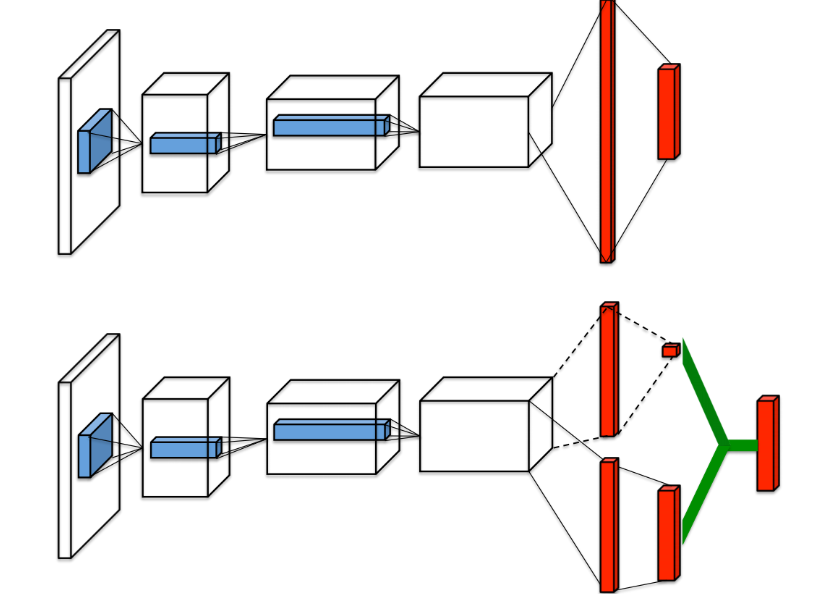
\includegraphics[width=0.5\linewidth]{figures/LiteratureStudy/RL_diagram_Dueling.png}
    \caption{\cite{wang2016dueling}. The top network is a standard Q-network, and the bottom network has a duelling architecture with two separate streams, the value and advantage streams.}
    \label{fig:enter-label}
\end{figure}

\subsubsection{Double Q-learning}
\label{sec:Double_Q_learning}

Standard DQNs tend to be biased towards over-optimistic value estimations due to the same Q-network selecting and evaluating the action. As a result, van Hasselt \cite{vanhasselt2016deep} proposed decoupling the selection and evaluation stages through a \textit{Double Q-network}, this showed to give better estimates and performances in complex environments.

These two Q-networks use the update rule of \autoref{eq:DoubleQLearning} where the leading network, parameters \(\theta\), is updated each iteration for action \(a_{t+1}\) selection, while the target network, parameters \(\theta^{-}\) evaluates these actions. After a set interval, the target network is updated to lower the over-estimation bias.

\begin{equation}
    Q(s_t, a_t; \theta) \leftarrow Q(s_t, a_t; \theta) + \alpha \left[ R(s_t, a_t) + \gamma Q(s_{t+1}, \arg\max_{a_{t+1}} Q(s_{t+1}, a_{t+1}; \theta); \theta^{-}) - Q(s_t, a_t; \theta) \right]
\label{eq:DoubleQLearning}
\end{equation}

\subsection{Replay buffers}
\label{sec:buffers}
Off-policy methods have increased sample efficiency through their ability to reuse experiences from previous transitions. For an environment like rocket landing where the manoeuvrer can take minutes leads to an episode with 1000s of steps when discretised by a modest 0.1s time step. Allowing the data to reused provides the agent with a broader range of experiences to update from is exploration is present. The \textit{replay buffer} holds the transition data such that they can be reused later on.

The first instance of the replay buffer was the \textbf{uniform replay buffer} used to play Atari games, \cite{mnih2013playing}, here transitions are stored in a First-In-First-Out manner with all samples having equal probability of being sampled to provide diverse training samples. The buffer stores the state, action, reward and next state for random batches of experiences to be sampled during training; this breaks the correlations of consecutive episodes.

\textbf{Prioritised Experience Replay} (PER) was then introduced to take actions with a better learning potential through sampling via their temporal difference (TD) error, \cite{schaul2015prioritized}. TD measures the prediction and target networks' Q-value differences, as shown in \autoref{eq:TD_error}. The immediate reward is summed with the future rewards (when active) and subtracted from the current Q-value estimate. A small constant is added to get the priority, with 'i' being the transition; this computes the probability $P(i)$. The hyperparameter $\tilde{\alpha}$ sets the importance of sampling previous transitions with a higher reward probability. The weights \(w_i\) are updated through \textit{importance sampling} where the hyperparameter $\tilde{\beta}$ determines the correction; trading off between faster learning and bias correction. 

\begin{equation}
\begin{aligned}
    e_{TD} =& |R(s_t, a_t) + (1 - \text{done}) \cdot \gamma \cdot \max_{a_{t+1}} Q(s_{t+1}, a_{t+1}; \theta^-) - Q(s_t, a_t; \theta)| \\
    \Tilde{p}_i =& e_{TD,i} + 10^{-5} \\
    P(i) =& \frac{p_i^{\alpha_{\text{PER}}}}{\sum_k p_k^{\alpha_{\text{PER}}}} \\
    w_i =& \left( \frac{1}{N \cdot P(i)} \right)^{\beta_{\text{PER}}}
\label{eq:TD_error}
\end{aligned}
\end{equation}

\textbf{Hindsight Experience Replay} (HER) is a goal-orientated replay buffer where an episode is replayed with a different goal the agent was trying to achieve. This replay buffer enhances learning efficiency for environments with sparse or delayed rewards. HER takes the states from failed episodes as alternative goals to generate valuable strategies for successful experiences. For example, if a robotic arm places an object in a different position, HER can leverage this as a new goal, leveraging failed trajectories to create additional data and improve sample efficiency. The algorithm to implement HER is shown in \cite{andrychowicz2017hindsight}.

\subsection{Exploration strategies}
\label{sec:exploration}

Exploration strategies balance the sensitive exploration and exploitation trade-off. Exploration is needed, especially in the early stages of learning a new part of the episode, to allow the agent to uncover new experiences which maximum the Q-value. Meanwhile, exploitation is also needed to force the agent to converge through taking the path with the maximum Q-value at that point.

Exploration strategies can be divided into two use cases: discrete spaces, $\epsilon$-greedy (\cite{sutton1998reinforcement}) and Boltzmann, and continuous spaces. For rocket landing, the state space (e.g., position, velocity, orientation) and the action space (e.g., thrust levels, gimbal angles) are continuous; as such only these strategies continuous strategies are covered.

\textbf{Action noise-based exploration} is an efficient way to encourage exploration in continuous space by adding noise.
\begin{itemize}
    \item \textit{Gaussian Noise}: in \cite{lillicrap2015continuous}, the exploration policy is created by adding random noise to the actor's policy. This is used in several actor-critic RL configurations used for learning on a continuous domain, like the Twin Delayed Deep Deterministic Policy Gradient (TD3) algorithm wrote in \autoref{sec:TD3}.

    \item \textit{Ornstein-Uhlenbeck (OU) noise}: is used to temporary correlate noise, \cite{lillicrap2015continuous} use this to enhance their exploration efficiency, showing it is good for "physical control problems with inertia".

    \item \textit{Adaptive Noise Scaling}: can be combined with a method above to balance exploration-exploitation during training. Here the noise is scaled is automatically altered, like in soft actor critic (SAC) shown in \autoref{sec:SAC}
\end{itemize}

\begin{tcolorbox}[title={\textbf{Lemma. Gaussian and OU noise}}]
Exploration in deterministic reinforcement learning methods like DDPG, D4PG or TD3 explained later in \autoref{sec:off_policy} requires the injection of external noise into the policy's action space to discover new and unseen solutions.  Two common types of noise processes are Gaussian and OU noise.

\textbf{Gaussian noise} is temporally uncorrelated and drawn independently at each timestep from a normal distribution. This noise is simple and suitable for environments where smoothness in action evolution over time is not critical.
\[
    \epsilon_t \sim \mathcal{N}(0, \sigma^2)
\]


\textbf{Ornstein–Uhlenbeck noise} introduces temporal correlation by modelling the stochasticity as mean-reverting process, meaning that the stochastic process tends to revert towards a long term mean. This mean-reverting proces temporally smooths noise, idea for physical control tasks with momentum like rocket landing where a sudden change in action can lead to instability. The correlation across timesteps simulates inertia, yielding more natural and consistent exploration trajectories.

\[
    \epsilon_{t+1} = \epsilon_t + \theta (\mu - \epsilon_t) \Delta t + \sigma \sqrt{\Delta t} \mathcal{N}(0, 1)
\]

Gaussian noise is simpler to implement than OU noise, however OU noise encourages smoother transitions in systems with momentum, like physical control tasks.
\end{tcolorbox}


\textbf{Parameter Space Noise} (PSN) was introduced to overcome the downfall of the action space noise of inconsistent exploratory behaviours due to a fixed state always giving different actions. This can give problems like early truncation where at points in the episode the action is sensitive to noise and needs to be precise. However, adaptive noise scaling to push the action space noise to small amounts at parts in the episode can overcome this problem. PSN adds noise through \autoref{eq:PSM} to perturb the policy network parameters at the start of each episode and maintain them fixed afterwards; this results in state-dependent actions, unlike Gaussian noise methods.

\begin{equation}
    \tilde{\theta} = \theta + \mathcal{N}(0, \sigma^2 \cdot I)
\label{eq:PSM}
\end{equation}

PSN has been experimented with in \cite{plappert2018parameter}, building on the work of \cite{sehnke2010parameter} and \cite{rucksties2008state}; they show PSN offers better exploration and avoids suboptimal converge on continuous environments, and has significant benefits in environments with sparse rewards, along with outperforming Evolutionary Strategies (ES).


In environments where extrinsic rewards are sparse, intrinsic rewards can allow the agent to explore better; this can be employed through an \textbf{Intrinsic Curiosity Module} (ICM) developed in \cite{pathak2017curiosity}, which encourages the agent to explore. Intrinsic rewards are provided by the agent's own experience, motivating them to explore without extrinsic rewards.

An inverse model, which predicts the action \(\hat{a}(s_t, s_{t+1})\), is trained via \autoref{eq:loss_ICM_inverse} to minimise the loss between the actual and predicted actions. The forward model predicts the next state's features \(\hat{\phi}_{s_{t+1}}(\phi_{s_t}, a_t)\), through minimisation in state feature prediction via \autoref{eq:loss_ICM_forward}. The intrinsic reward, \autoref{eq:intrinisic_reward}, depends on the hyperparameter $\eta$ acting as the scaling factor. The total resulting reward is the sum of the extrinsic and intrinsic rewards.

\begin{equation}
    L_I(\hat{a}_t, a_t; \theta^I) = -\log P(a_t | s_t, s_{t+1}; \theta^I)
\label{eq:loss_ICM_inverse}
\end{equation}

\begin{equation}
    L_F(\phi(s_t), \hat{\phi}(s_{t+1}; \theta^F)) = \frac{1}{2} \|\phi(s_{t+1}) - \hat{\phi}(s_{t+1}; \theta^F)\|^2
\label{eq:loss_ICM_forward}
\end{equation}

\begin{equation}
    R^{\text{intrinsic}}_t = \eta \cdot \frac{1}{2} \|\phi(s_{t+1}) - \hat{\phi}(s_{t+1}; \theta^F)\|^2
\label{eq:intrinisic_reward}
\end{equation}

An alternative to ICM is \textbf{Random Network Distillation} (RND), introduced in \cite{burda2018exploration}, where they argue it is simpler and more stable than ICM, through testing on Montezuma's Revenge. This method works well for sparse reward environments, allowing extrinsic and intrinsic rewards to be flexibly combined. Here, intrinsic rewards are based upon a prediction error from a trainable "prediction" network approximating a fixed and randomly initialised "target" network. The prediction network is trained to minimise the prediction error through \autoref{eq:RND_1}. The intrinsic reward can be set equal to the prediction network loss, as such states explored less will gain a higher prediction error, and thus, the RND encourages them to be explored; this process is visualised in \autoref{fig:RND}. In essence, RND measures how novel a state is by comparing prediction error on a fixed random target network.

\begin{equation}
    L_{\text{predict}} = \frac{1}{2} \cdot ||y_{\text{target}} - y_{\text{predict}} ||^2 = r_{\text{intrinsic}}
\label{eq:RND_1}
\end{equation}

\begin{figure}[H]
    \centering
    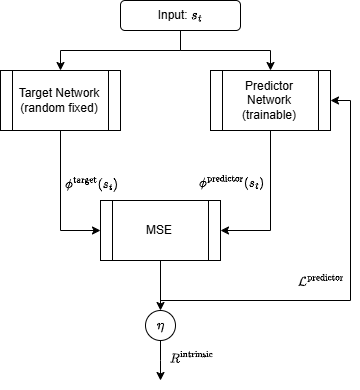
\includegraphics[width=0.5\linewidth]{figures/LiteratureStudy/RL_diagram_RND.png}
    \caption{Flow diagram showing how RND works.}
    \label{fig:RND}
\end{figure}

\textbf{Noisy networks} (\cite{fortunato2017noisy}) incorporate parametric noise into the network weights to enhance exploration efficiency via stochastic diversity of the agent's policy. Here, Stochastic Gradient Descent (SGD) learns the noise scale, adapting it over time; for instance, less noise is present as the agent becomes more confident, decreasing exploration. The authors also show how it is compatible with any RL architecture which employs SGD. Ultimately arguing, noisy networks provide structured and adaptive exploration.

\subsection{Off-Policy Continuous On-Line Methods}
\label{sec:off_policy}
As reasoned in \autoref{sec:ICS} an online offpolicy method which works with a continuous action and observation space is the chosen method due to its sample efficiency. The actor-critic framework is the commonly used to learn an optimal policy for online and continuous domain problems. The actor learns the optimal policy by Q-value maximisation; maximising the expected cumulative return from taking a given action in a given state. So the actor, \(\zeta(s_t; \theta^Z)\), learns the action for each state to maximise expected return through \autoref{eq:maxQ_AC}, with the mapping of state to action learnt through a neural network acting as a function approximator. The critic estimates the state-action value \(Q(s_t, a_t; \theta^Q)\); the expected reward for taking an action in a given state, this is used by the actor to update its policy. The critic is used instead of raw rewards to train the actor because it reduces the variance of policy gradient updates by providing smoothed action-value estimates.

Meanwhile, the critic learns to minimise TD error \footnote{Defined in \autoref{sec:exploration}.}. For example, \autoref{eq:TD_AC} shows the scenairo for a critic where the TD error between the predicted state-action pair and the critic's target network.

\begin{equation}
    \mathcal{L}_Q(\theta^Q) = \frac{1}{N_{\text{buffer}}} \cdot \sum_{i=1}^{N_{\text{buffer}}}(R^i(s^i_t, a^i_t) + \gamma \cdot Q'(s^i_{t+1}, \zeta'(s^i_{t+1};\theta^{\zeta'});\theta^{Q'}) - Q(s^i_t, a^i_t; \theta^Q))^2
\label{eq:TD_AC}
\end{equation}

\begin{equation}
    \mathcal{L}_\zeta(\theta^\zeta) = - \frac{1}{N_\text{buffer}} \cdot \sum_{i=1}^{N_{\text{buffer}}} Q(s^i_t, \zeta(s^i_t;\theta^\zeta);\theta^Q)
\label{eq:maxQ_AC}
\end{equation}

The following subsections cover 5 of the main continuous online offpolicy reinforcement  learning algorithms found in literature. SAC and Maximum a posteriori Policy Optimisation (MPO) learn a stochastic policy, while Deep Deterministic Policy Gradient (DDPG), Distributed Distributional Deterministic Policy Gradient (D4PG) and TD3 learn a deterministic policy.

\subsubsection{Deep Deterministic Policy Gradient method}
\label{sec:DDPG}

DQNs work with a discrete action space, as such with a continuous control problem the continuous outputs have to be discretised leading to massive a massive action dimension, inhibiting learning. DDPG was presented by \cite{lillicrap2015continuous} to be a solution to this problem through an extension to the Deterministic Policy Gradient (DPG) method (\cite{silver2014deterministic}), allowing for a model-free offpolicy online actor-critic algorithm with neural networks utilised as deep function approximators to learn a policy and state-action value function in continuous domains.

The actor provides deterministic actions with the critic approximating the resulting Q-value. \cite{mnih2015human} utilise target networks and experience replay, like in DQNs, to stabilise training and improve sample efficiency, and OU noise is used for action noise-based exploration like explained in \autoref{sec:exploration}.

To summarise DDPG is an actor-critic framework with extensions being:
\begin{enumerate}
    \item Action-space-based noise used for exploration.
    \item Target networks used to improve learning stability, through Polyak averaging \autoref{eq:target_networks}.
\begin{equation}
\begin{aligned}
    \theta^{Q'} \leftarrow& \tilde{\tau} \cdot \theta^Q + (1 - \tilde{\tau}) \cdot \theta^{Q'}\\
    \theta^{\zeta'} \leftarrow& \tilde{\tau} \cdot \theta^\zeta + (1 - \tilde{\tau}) \cdot \theta^{\zeta'}
\end{aligned}
\label{eq:target_networks}
\end{equation}
    \item A replay buffer \(\mathcal{R}\) for off-policy learning, improving sample efficiency.
\end{enumerate}

\begin{tcolorbox}[title={\textbf{Lemma. Target network updates via Polyak averaging}}]
In deep reinforcement learning tasks target networks are often used to stabilise learning by slowly the changing of targets used for value estimation. Instead of directly copying the online netwrok's weights, they are soft updated through \textit{Polyak averaging}..

employed to stabilise learning by providing slowly changing targets for value estimation. Instead of directly copying the online network's weights to the target network, a soft update method called \textit{Polyak averaging} is used.

Let \( \theta \) denote the parameters of the online network and \( \theta^{'}\) the parameters of the corresponding target network. The Polyak update rule is defined as:
\[
    \theta^{'} \leftarrow \tau \theta + (1 - \tau) \theta^{'} 
\]
where \( \tau \in (0, 1) \) is the averaging coefficient, a larger coefficient tracks the target network faster and can induce instability. Alternatively, a small coefficient gives stable but slower updates which can enhance robustness.

Polyak averaging ensures the parameters of the target network move slowly towards that of the online network, reducing oscillations and divergence in value estimation, to promote learning stability.
\end{tcolorbox}

\subsubsection{Distributed Distributional Deterministic Policy Gradients}
\label{sec:D4PG}

\cite{barthmaron2018d4pg} extended DDPG to D4PG to include a distributional critic promotes learning stability, along with PER for faster learning and N-step returns for improving the rewards over longer-time horizons.
\begin{itemize}
    \item A distributed framework is used, where multiple actors asynchronously generate experiences and fill a shared replay buffer, where a central learner updates the policy.
    \item A \textit{distributional critic} is used, essentially instead of modelling a scalar \(Q(s,a; \theta^Q)\) it predicts a probability distribution \(Q_Z(s,a; \theta^{Q_Z})\) over all possible returns, this distribution modelling works well for stochastic environments where differing Q values can come from different actions in the same state. The critic now outputs a probability distribution leading to KL divergence used instead of MSE for the loss function.
    \item N-steps are used to give the reward over a longer time horizon, this is beneficial for task where there are long-term dependencies, such as in rocket landing. The N-step reward equation is shown in \autoref{eq:N_step_rewards}.
\end{itemize}

\begin{equation}
    y^i_t = \bigg(\sum_{m=0}^{N_{\text{episode}}} \gamma^m \cdot R(a^i_m, s^i_m)\bigg) + \gamma^{N_{\text{episode}}} \cdot Q_Z'(s^i_{N_{\text{episode}}}, \zeta'(s^i_{N_{\text{episode}}}; \theta^{\zeta'}); \theta^{Q'})
\label{eq:N_step_rewards}
\end{equation}

\begin{tcolorbox}[title={\textbf{Lemma. N-step returns}}]
In traditional TD learning the value estimate of a state is updated based on the immediate reward and the estimated discounted value of the next state. \autoref{eq:one_step_rewards} is the equation for calculated the 1-step return at time t ($G_t^{(1)}$ ) using the immediate reward ($R_{t+1}$) and the estimated value of the next state ($V(s_{t+1})$).

% $G_t^{(1)}$ is the 1-step return at time t
% $R_{t+1}$ is the immediate reward
% $\gamma$ is the discount factor
% $V(S_{t+1})$ is the estimated value of the next state

\begin{equation}
    G_t^{(1)} = R_{t+1} + \gamma V(s_{t+1})
\label{eq:one_step_rewards}
\end{equation}

N-step returns extends this concept to look ahead $n$ steps through \textit{booststrapping} the fine value estimate.ping. \autoref{eq:n_step_rewards} shows the generic formula for n-step rewards. N-step returns allows the agent to learn from a longer sequence of rewards before bootstrapping, giving it more information about long-term dependencies

\begin{equation}
    G_t^{(n)} = R_{t+1} + \gamma R_{t+2} + \gamma^2 R_{t+3} + ... + \gamma^{n-1} R_{t+n} + \gamma^n V(S_{t+n})
\label{eq:n_step_rewards}
\end{equation}

This formula changes when terminal states are within the trajectory length set for n-step returns ($n$), otherwise called within the n-step horizon. The returns should only include rewards up to the terminal state, either a truncated or completed episode, with no bootstrapping or rewards after termination. If step $t+k$ is a terminal state,where $k < n$), the n-step return becomes \autoref{eq:n_step_rewards_terminal}.

\begin{equation}
    G_t^{(n)} = R_{t+1} + \gamma R_{t+2} + ... + \gamma^{k-1} R_{t+k}
\label{eq:n_step_rewards_terminal}
\end{equation}
\end{tcolorbox}

\subsubsection{Twin Delayed DDPG}
\label{sec:TD3}


\cite{fujimoto2018addressing} use double Q-learning in an actor-critic format to reduce overestimation bias of the value function through a pair of independent critics and double Q-learning. Through their approach, they run DDPG with two extensions:
\begin{enumerate}
    \item Clipped Gaussian noise is used instead of OU for action space-based noise; clipped noise is chosen to prevent sharp action value changes causing over-fitting.
    \item Through the use of double Q-learning (dual critics), the loss functions for the critic have the "target critic changed" to the minimum between the networks, ensuring the most conservative estimate. For the actor loss, only the primary Q-network is considered; this ensures it is based on a single Q-value estimate reducing noise and learning instability.
\end{enumerate}

\subsubsection{Soft Actor-Critic}
\label{sec:SAC}

\cite{haarnoja2018soft} introduce SAC as an actor-critic algorithm which maximises both expected rewards and the policy's entropy, encouraging exploration and thus leading to more robust policies. 
TD3 uses Gaussian action space noise, whereas SAC's actor outputs a Gaussian distribution \(\zeta_S(s;\theta^{\tilde{\zeta}}, \theta^\mu, \theta^\sigma)\), with the subscript "S" denoting it as a stochastic actor. This actor outputs \(\mu(s_t; \theta^\mu)\) and \(\sigma(s_t; \theta^\mu)\), which are converted to a noisy action through \autoref{eq:SAC_actor}. Compared to TD3, the difference is that the noise distribution is a learned parameter providing \textit{state-dependent exploration}.

\begin{equation}
\begin{aligned}
    \sigma(s; \theta^\mu) = e^{\log \sigma(s; \theta^\mu)} ,\quad
    \tilde{a} = \mu(s; \theta^\mu) + \sigma(s; \theta^\mu) \odot \epsilon ,\quad
    \epsilon \sim \mathcal{N}(0,I) ,\quad
    a = tanh(\tilde{a})
\end{aligned}
\label{eq:SAC_actor}
\end{equation}

\begin{figure}[H]
    \centering
    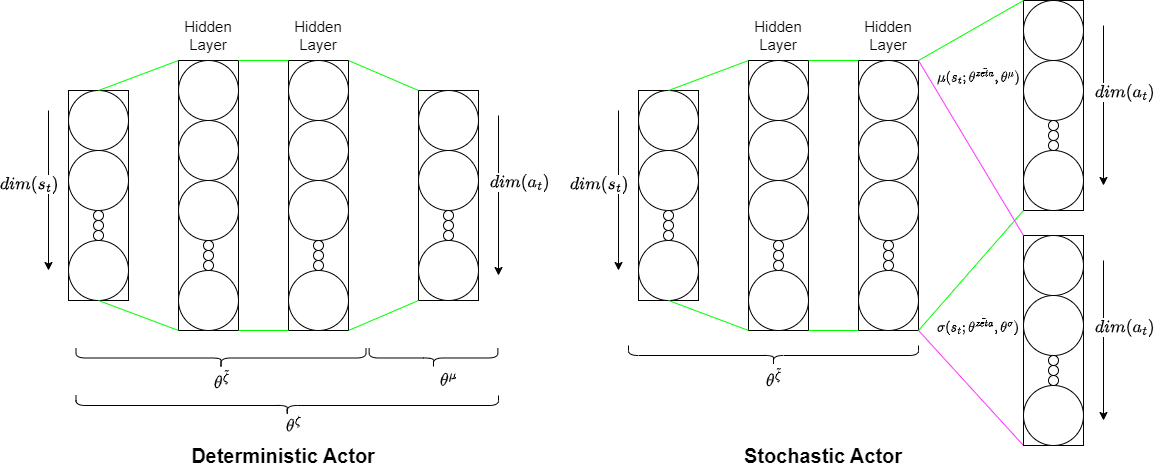
\includegraphics[width=0.95\linewidth]{figures/LiteratureStudy/RL_diagram_ActorNetworks.png}
    \caption{Diagram showing the differences in actor networks, for deterministic and stochastic.}
    \label{fig:actor_networks}
\end{figure}

SAC has an additional entropy term to control the state-dependent exploration. \textit{Temperature} $v$ updates to encourage an entropy to meet the target entropy controlling the degree of randomness and traditionally set as  \(\mathcal{H}_{\text{target}} := -\dim(a_t)\). \autoref{eq:SAC_temperature} temperature is updated to encourage the negative Gaussian likelihood equal to the target entropy.

\begin{equation}
    \mathcal{L}_{\log(\nu)} = \frac{1}{N} \cdot \sum_{i=1}^{N}-\log(\nu) \cdot \bigg(\log p(a_t^i|\mu,\sigma^2)+\mathcal{H}_{\text{target}}\bigg)
\label{eq:SAC_temperature}
\end{equation}


\begin{tcolorbox}[title={\textbf{Lemma. Gaussian likelihood}}]
The Gaussian likelihood is the probability density function of a normal distribution evaluated at a given point. For a random variable \( x \in \mathbb{R}^d \), with mean \( \mu \in \mathbb{R}^d \) and standard deviation \( \sigma \in \mathbb{R}^d \), the log-likelihood is given by:
\[
\log p(x \mid \mu, \sigma^2) = -\frac{1}{2} \left[ \frac{(x - \mu)^2}{\sigma^2} + 2 \log \sigma + \log(2\pi) \right]
\]
The Gaussian likelihood shows how likely point $x$ is under the $\mu$ and $\sigma^2$. The first term is called the \textit{quadratic term} and penalises deviations from the mean scaled by the variance. The second term called the \textit{normalisation term} accounts for the distribution spread, and the final term is a constant ensuring proper normalisation.

A lower negative log probability, \textit{Gaussian likelihood}, indicates the sample is more likely under the distribution, while a high negative log probability indicates a less likely sample under the distribution.
\end{tcolorbox}

The actor has two terms in its loss function, first an entropy regularisation term, where the log probability gives a metric for the likelihood of the actor, weighted by the temperature. The temperature updates previously to balance entropy through changing the entropy regularisation loss magnitude in the reward function. The second term extracts the minimum of two q network outputs, alike double q-learning, to reduce overestimation bias; this term encourages the policy to select the actions of that state with the highest expected returns.

\begin{equation}
    \mathcal{L}_{\zeta^S} = \frac{1}{N} \cdot \sum^N_{i=1} \bigg(\nu \cdot \log p(a_t^i|\mu, \sigma^2) - \min_{i=1,2}Q(s_t^i,a_t^i;\theta^{Q_i})\bigg)
\label{eq:SAC_actorloss}
\end{equation}

The TD error is computed to represent the mean-squared Bellman error for each critic, which is trained to minimised the square difference between its predicted Q-value and the shared TD target, through the loss function of \autoref{eq:SAC_critic_loss}.

\begin{equation}
\begin{aligned}
    TD_{\text{target}} =& R_t + \gamma \cdot (1-d) \cdot \bigg(\min_{i=1,2} \{Q'(s',a';\theta^{Q'})\}- \nu \cdot \log p(a'|\mu',(\sigma')^2)\bigg) \\
    e_{TD} =& \frac{1}{2} \cdot \bigg((TD_{\text{target}} - Q_1)^2 + (TD_{\text{target}} - Q_2)^2\bigg)
\end{aligned}
\label{eq:TD_error_entropy_regularised}
\end{equation}

\begin{equation}
    \mathcal{L}_Q = \frac{1}{N} \cdot \sum^N e_{TD}
\label{eq:SAC_critic_loss}
\end{equation}

% SAC in a distributed format
SAC has been used to perform many tasks, \cite{wahid2020learning} used it in a distributed form to perform control and navigation tasks. While \cite{akimov2019distributed} used it in a distributed framework to update a shared replay buffer and used a multivariate reward representation to have sub-rewards allowing for transfer learning, which utilises knowledge distillation to increase learning speed.

% STOPPED HERE
\subsubsection{Maximum a posteriori Policy Optimisation}
\label{sec:MPO}

\cite{schulman2015trpo} introduced Trust Region Policy Optimisation (TRPO) as an iterative procedure for policy optimisation suitable to large non-linear policies of neural networks. Here a trust region controls the update between policies through Kullback-Leibler (KL) divergence. \cite{schulman2017proximal} presented Proximal Policy Optimisation (PPO) as a first-order approximation of the second-order optimisation TRPO. The paper states have PPO is simler, more generic and of better sample efficiency than TRPO, and consistently outperforms other onpolicy online methods like Advantage Actor-Critic (A2C).

PPO is a stochastic actor-critic framework which prevents large updates causing instability through constraints on the deviation of the policy through their KL divergence.

\begin{tcolorbox}[title={\textbf{Lemma. KL divergence}}]
The KL divergence is a measure of how one probability distribution \( P \) diverges from a second, reference distribution \( Q \). For continuous distributions with probability densities \( p(x) \) and \( q(x) \), the KL divergence from \( Q \) to \( P \) is defined as:
\[
\mathcal{D}_{\mathrm{KL}}(P \parallel Q) = \int p(x) \log \frac{p(x)}{q(x)} \, dx
\]
The smaller the KL divergence the more identical the distributions are.
\end{tcolorbox}

PPO was first employed without a value function, where the advantage estimate \(\hat{A}_t\) is equal to the Monte Carlo return \(G_t(s_t, a_t) = \sum_{k=0}^\infty \gamma^k \cdot R_{t+k}(s_t, a_t) \). From here, a clipped surrogate objective is used to update the policy, as shown through the second equation in \autoref{eq:PPO}. Note that the other objectives, including a KL divergence-based penalty, were used and showed decreased performance.

\begin{equation}
\begin{aligned}
    \text{No clipping or penalty:}& \mathcal{L}(\theta) = r_t(\theta) \cdot \hat{A}_t(s_t, a_t) \\
    \text{Clipped:}& \mathcal{L}(\theta) = \min\{r_t(\theta)\cdot\hat{A}_t(s_t, a_t), \text{clip}(r_t(\theta), 1 - \epsilon^{\text{PPO}}, 1 + \epsilon^{\text{PPO}}) \cdot \hat{A}_t(s_t, a_t) \\
    \text{KL penalty:}& \mathcal{L}(\theta) = r_t(\theta) \cdot \hat{A}_t(s_t, a_t) - \beta^{\text{PPO}} \cdot \text{KL}[\zeta_{\text{old}}(s_t; \theta^{\zeta_{\text{old}}}) || \zeta(s_t; \theta^\zeta)] \\
    \text{With:}& r_t(\theta) = \frac{\zeta(s_t; \theta^\zeta)}{\zeta_{\text{old}}(s_t; \theta^{\zeta_{\text{old}}})}
\end{aligned}
\label{eq:PPO}
\end{equation}

The actor-critic PPO was introduced to improve sample efficiency via value function estimation to stabilise the advantage function estimate by \autoref{eq:PPO_critic}. Here, the critic is trained to minimise the value loss through MSE \(MSE[G_t, V_t]\).

\begin{equation}
\begin{aligned}
    G_t(s_t, a_t) =& \sum_{k=0}^\infty \gamma^k \cdot R_{t+k}(s_t, a_t) \\
    A_t(s_t, a_t) =& G_t(s_t, a_t) - V(s_t; \theta^\zeta) \\
\end{aligned}
\label{eq:PPO_critic}
\end{equation}

%MPO
\cite{abdolmaleki2018maximum} introduce MPO as an off-policy version to PPO, which has better sample efficiency. They state it boasts the robustness, insensitivity to hyperparameter changes, and scalability of an on-policy algorithm while having the off-policy sample efficiency due to their utilisation of a replay buffer. MPO decouples PPO into two steps:
\begin{enumerate}
    \item Optimisation of a non-parametric target policy.
    \begin{itemize}
        \item The intermediate policy with a probabilistic representation of the value function.
        \item \(\nu\) controls the steepness of distribution, in essence controlling the exploration-exploitation trade-off.
        \item It doesn't rely on a neural network and is computed for the value function, acting like a "soft target" or a reference policy.
    \end{itemize}
    \item Parametric policy updating for target approximation.
    \begin{itemize}
        \item The actual policy which the agent uses to interact with the environment, parametrised through a neural network.
        \item Updates through minimisation of the KL divergence with its non-parametric policy.
    \end{itemize}
\end{enumerate}

The target policy is updated through \autoref{eq:Estep} called the \textit{E-Step} (expectation step). Note that the actor is stochastic, like SAC.

\begin{equation}
    \zeta_{\text{S, target}}(s_t; \theta^{\zeta_{\text{target}}}) \varpropto  \exp\left(\frac{Q(s, a)}{\nu}\right)
\label{eq:Estep}
\end{equation}

The parametric policy is updated through minimisation of the KL divergence of the target and parametric network, as shown in \autoref{eq:PPO}, incorporating  KL divergence constraint to stay within the trust region. Meanwhile, the critic is updated as normal.

The temperature parameter is updated through dual optimisation of \autoref{eq:MPO_dual}, here \(\epsilon^\nu\) controls the variance of the weights for regularisation. \cite{prior2024jaxrl}, use Sequential Least Squares Programming (SLSQP) is used to minimise the dual function concerning $\nu$, with a softmax function used to normalise the new weights, \autoref{eq:MPO_softmax}.


\begin{equation}
    g(\eta) = \nu \cdot \epsilon^{\nu} + \eta \cdot [\mathbb{E}_{s\sim R}[\log(\frac{1}{N_{\text{buffer}}}\cdot\sum_{i=1}^{N_{\text{buffer}}}\exp(\frac{Q(s, a_i; \theta^Q)}{\nu^*}))]]
\label{eq:MPO_dual}
\end{equation}

\begin{equation}
    w_i = \frac{\exp(\frac{Q(s, a_i)}{\eta})}{\sum_j \exp(\frac{Q(s, a_j)}{\eta})}
\label{eq:MPO_softmax}
\end{equation}

The actor updates through the log-likelihood of the target and current policies, as is a multi-variate Gaussian distribution. Secondly, it has two Lagrangian multipliers \(\lambda^\mu\) and \(\lambda^\sigma\) to maintain the constraints on the KL divergence between the target and current policy's Gaussian distributions. Pre-defined thresholds \(M^\mu\) and \(M^\sigma\) define the \textit{trust region}. This process is shown in \autoref{eq:MPO_actor}.

\begin{equation}
\begin{aligned}
    \mathcal{L}^\sigma &= \lambda^\sigma \cdot \left(M^\sigma - D_{KL}(\zeta^{\text{target}}(s_t; \theta^\sigma) \parallel \zeta(s_t; \theta^\sigma))\right), \\
    \mathcal{L}^\mu &= \lambda^\mu \cdot \left(M^\mu - D_{KL}(\zeta^{\text{target}}(s_t; \theta^\mu) \parallel \zeta(s_t; \theta^\mu))\right), \\
    \mathcal{L}^{\zeta, \text{unconstrained}} &= - \frac{1}{N^{\text{buffer}}} \sum_{i=1}^{N^{\text{buffer}}} \Big( \log P(a_i \mid \mu^{\text{target}}(s_t; \theta^\mu), \sigma(s_t; \theta^\sigma)) \\
    &\quad + \log P(a_i \mid \mu(s_t; \theta^\mu), \sigma^{\text{target}}(s_t; \theta^{\sigma^{\text{target}}})) \Big).
\end{aligned}
\label{eq:MPO_actor}
\end{equation}


The \textit{"Maximum a Posteriori"} framework balances the exploration-exploitation trade-off through a trust region. Like SAC, a temperature parameter \(\nu\) controls the system's entropy. The authors tested it on control tasks \textit{Walker-2D}, \textit{Acrobat}, and \textit{Hopper}; it was shown to outperform DDPG and PPO in an extensive ablation study. However, there is limited evidence of whether it can outperform more advanced DDPG algorithms like D4PG, SAC or TD3.

\cite{prior2024jaxrl} implement this scheme in JAX (\cite{jax2018github}) with a double critic alike TD3. Deduced to be used to reduce overestimation bias; secondly, they clip the gradient of the loss function for the actor update. Finally, target networks are used.

The original paper runs the MPO algorithm in a distributed form, with a single learner but multiple learners (agents) collecting data independently, with a \text{chief} collecting the gradients and performing a parameter update through averaging gradients. In other words, \textit{distributed synchronous SGD}.


Finally, MPO can be used in a distributed framework, with the user able to configure it however they like. \cite{hoffman2020acme} implemented DMPO in their Acme framework, using distributional critics similar to D4PG.

\subsection{Normalisation functions}
\label{sec:normalisation_functions}
Normalisation can be applied to observations, actions and rewards to stabilise training and brining values within the same range. ADD MORE MOTIVATION. In this section different types of normalisation shall be presented.

$\mathbf{\tanh}$ \textbf{normalisation:} smooths saturation of large values to squish outliers between $(-1,1)$. The $k$ factor can be selected to give the maximum expected value equal to an output of say 0.8, such that there is room for outliers beyond on that.

\begin{equation}
    x' = \tanh(k \cdot x)
\end{equation}

\textbf{Min-max normalisation:} is a simple linear scaling, which is interpretable, but is sensitive to outliers.

\begin{equation}
    x' = \frac{x - \min(x)}{\min(x) - \max(x)}
\end{equation}

\textbf{Shifted normalisation:} zero centers the data but does not reduce it to within a range.

\begin{equation}
    x' = x - \mu(x)
\end{equation}

\textbf{Exponential scaling:} amplifies large value while suppresses small values to increase contrast. This can be useful for some scenarios where reward shaping wants large values to be emphasized.

\begin{equation}
    x' = e^{k \cdot x}
\end{equation}

\textbf{Logarithmic scaling:} is used to compress large values and expand small ones to reduce the dynamic range. It is useful to stabilise large-magnitude inputs, providing an alternative to $\tanh$ and clipping. Also, it can be bounded to between 0 and 1 through its denominator.

\begin{equation}
    x' = \frac{\log(1 + x)}{\log(1 + \max(x))}
\end{equation}

\subsection{Reinforcement learning algorithm selection}
\label{sec:RL_algo_selection}
The reinforcement learning section of the literature study has covered key concepts in online offpolicy reinforcement learning algorithms. In terms of learning for a physical control task, the rocket will need state-dependent exploration to ensure no sudden changes in action and at times a lower noise when the action is sensitive. For instance when travelling near the dynamic pressure limit of the rocket the grid fin angles will be more sensitive to a change in state than for at lower angles. Furthermore, the injected noise should scale with the magnitude of the mean action, since for example the physical effect of a deviation from a small gimbal angle is less significant than the same deviation at larger angles.

OU noise performs better than Gaussian noise to prevent sudden changes as is a mean-reverting process. However, MPO and SAC have a trainable stochastic network allowing for state-dependent exploration. As such, MPO and SAC are the two chosen algorithms. ICM and RND at intrinisic rewards to the network, which is beneficial in sparse environments, but if the reward function during landing is set to increase extrinisic rewards it diminishes the need for these and reduces the number of learnable parameters. Noisy networks and PSN provide exploration through injecting noise into the weights of the network, this will only be trialled if the exploration from the selected RL algorithm is insufficient.

% Buffer
As an offpolicy methods requires the ability to reuse experiences from previous transitions, these must be stored in a buffer. \autoref{sec:buffers} covers three types of buffer, first the simple uniform replay buffer to randomly sample transitions, then the PER which focuses on action with better learning potential, and finally HER a goal-orientated buffer enhancing learning efficiency for environments with sparse or delayed rewards. As set previously, the reward function will be non-sparse, giving HER to have limited benefit. The implementation of PER can be based on a uniform buffer's code skeleton, so the algorithm can have the option to set both a uniform and prioritised replay buffer.

% N-step rewards
In D4PG Barth-Maron use N-step rewards to change the value estimate from using only immediate reward and the estimated value of the next step to n-step returns. Here the reward is propagated over multiple steps before bootstrapping the value network. A richer and temporally extended learning signal is provided, which will benefit the rocket in working with delayed rewards through enhancement of credit assignment over the trajectory.

In the context of a landing rocket, this scenairo could be avoiding maximum dynamic pressure, as the maximum dynamic pressure a rocket reaches is dependent on the previous actions taken of the whole trajectory rather than the only the final action before the limit is reached. Also, for it allows for the terminal reward to be propagated throughout the trajectory.

The trade-off is that N-step returns other a more informative reward to promote learning efficiency but increase the variance of the rewards, as such it is important to scale the reward assigned through \autoref{eq:n-step-scaling-factor} to take into account n-step propagation. The trajectory length chosen must be long enough to propagate the rewards, but if it is too long it will increase variance. A trajectory length which is too long can be discovered through a high variance on sampled rewards from the buffer or a large kurtosis, along with the critic struggling to reduce TD errors.

\begin{equation}
    R_t = R_t \cdot \frac{1-\gamma}{1-\gamma^n}
\label{eq:n-step-scaling-factor}
\end{equation}

The trade-off is that N-step methods may increase variance, but this is typically offset by improved learning efficiency when combined with experience replay. The use of off-policy algorithms like SAC and MPO makes this compatible with replay buffers, allowing for stable N-step learning from past transitions.

\begin{tcolorbox}[title={\textbf{Lemma. N-step reward scaling factor}}]
To ensure consistency in the magnitude of returns between 1-step and n-step temporal difference updates, the n-step rewards must be scaled appropriately. Consider the case where the per-step reward \( R \) is constant. The n-step return becomes:
\[
G_t^{(n)} = \sum_{k=0}^{n-1} \gamma^k R = R \cdot \sum_{k=0}^{n-1} \gamma^k
\]
This is a finite geometric series and evaluates to:
\[
G_t^{(n)} = R \cdot \frac{1 - \gamma^n}{1 - \gamma}
\]
To match the scale of a 1-step reward, the reward at each step can be rescaled by the inverse of the geometric sum:
\[
R_t^{\text{scaled}} = R_t \cdot \frac{1 - \gamma}{1 - \gamma^n}
\]
This correction ensures the total magnitude of accumulated rewards remains consistent across different choices of \( n \), reducing instability from overly large return targets in long-horizon settings.
\end{tcolorbox}

% L2 regularisation
Regularisation is technique used in machine learning to reduce a networks overfitting and encourage its ability to generalise. In terms of a critic this can cause the critic to overfit to reduce a few outlying large TD errors reducing its generalisability to the rest of the data. As for the actor, it can generalise well for specific states, but struggles in new unseen scenairos. To regularise the critic L2 regularisation (\cite{krogh1992weightdecay}), otherwise known as weight decay, shall be used to discourage large weights.

\begin{tcolorbox}[title={\textbf{Lemma. L2 regularisation (weight decay)}}]
L2 regularisation improves the generalisation of neural networks by penalising large weight magnitudes, through a quadratic penalty term added to the loss function, modifying the loss to:

\[
\mathcal{L}_{\text{total}} = \mathcal{L}_{\text{original}} + \lambda \lVert \theta \rVert_2^2
\]
where \( \lambda \) is a L2 regularisation coefficient hyperparameter controller the strength of the regularisation. This penalty encourages the optimiser to find small-weight solutions; which become less sensitive to noise and decrease likelihood of overfitting. Empirical evidence from Krogh and Hertz (1992) supports the effectiveness of L2 regularisation in improving generalisation across a wide range of tasks.
\end{tcolorbox}

\cite{andrychowicz2020matters} investigated the impact of different normalisation techniques, a form of regularisation. First they showed how input normalisation benefits most RL environments. For an environment like rocket landing were altitude can vary tens of thousands of meters and pitch angle to a few degrees, input normalisation is required. As the critic takes in both action and observation, both need to be normalised. To bound the states, they will be normalised between -1 and 1 through selected normalisation functions per state, by \autoref{sec:normalisation_functions}. The actor's network outputs will be bounded a $\tanh$ activation function to ensure the mean is $\in (-1,1)$ which can then be scaled to the resulting action, through functions of the inverse of \autoref{sec:normalisation_functions}.

They also review gradient clipping, although they note it of secondary importance, they show it does benefit learning stability. Here the magnitude of gradients of backpropagation are bounded 
to provide a safety net against exploding gradients, needed in high-variance environments, which could occur with the use of n-step rewards. Finally, reward normalisation will take place to reduce the variance of rewards and ensure no drastic changes in reward throughout the episode.

\begin{tcolorbox}[title={\textbf{Lemma. Gradient clipping (global norm scaling)}}]
Gradient clipping regularises training through prevention of gradient explosion to stabilise it through bounding the update step. The global L2 norm of all gradients across the network is computed:
\[
\lVert g \rVert = \sqrt{ \sum_i \sum_j g_{ij}^2 }
\]
If this norm exceeds a user-defined threshold \( \tau \), all gradients are scaled uniformly by a factor:
\[
\text{scale} = \min\left(1, \frac{\tau}{\lVert g \rVert + \varepsilon} \right)
\]
where \( \varepsilon \) is a small constant added for numerical stability. Each parameter's gradient \( g_i \) is then rescaled:
\[
g_i \leftarrow g_i \cdot \text{scale}
\]
\end{tcolorbox}

% MPO vs. SAC